%\documentclass[spanish]{beamer}
\documentclass{beamer}
\usepackage{pgf,pgfpages}
%\pgfpagesuselayout{4 on 1}[letterpaper,landscape,border shrink=0.5in]
\usepackage{algorithm,algorithmic}
%\usepackage{algorithm,algorithmicx}
%\usepackage[noend]{algpseudocode}
\usepackage{listings}
\lstset{basicstyle=\ttfamily,
	showstringspaces=false,
	commentstyle=\color{red},
	literate={á}{{\'a}}1
	{ã}{{\~a}}1
	{é}{{\'e}}1
	{É}{{\'E}}1
	{ó}{{\'o}}1
	{í}{{\'i}}1
	{ñ}{{\~n}}1
	{¡}{{!`}}1
	{¿}{{?`}}1
	{ú}{{\'u}}1
	{Í}{{\'I}}1
	{Ó}{{\'O}}1
}

\usepackage{beamerthemesplit}
\usepackage{color}
\usepackage[utf8]{inputenc}
\usepackage[spanish]{babel}
%\usepackage[latin1]{inputenc}
%\usepackage[pdftex]{graphicx}
%\usepackage{algorithm}
%\usepackage{algorithmic-C}
%\usepackage{algorithmic}
\usepackage{amsthm}
\usepackage{multicol}
\usepackage{multirow}
\usepackage{fancyvrb,relsize}
\usepackage{hhline}
\usepackage{tikz}
\usetikzlibrary{trees, shapes, calc}
\newcommand{\inputTikZ}[2]{%
	\scalebox{#1}{\input{#2}}
}

\usetheme{Warsaw} %Gueno
%\usetheme{Darmstadt} %OK!
% \usetheme{Frankfurt} %OK!
%\usetheme{Goettingen}
%\usetheme{Dresden}
%\usetheme{JuanLesPins} %OK!!
%\usetheme{Marburg}
%\usetheme{Montpellier}
%\usetheme{Rochester} %sobrio
%\usetheme{Singapore}
%\usetheme{Szeged}

%\usecolortheme{albatross}
%\usecolortheme{seahorse}
%\usecolortheme{beetle}
%\usecolortheme{crane}
%\usecolortheme{dolphin}
%\usecolortheme{dove}
%\usecolortheme{fly}
%\usecolortheme{lily} %Gueno
\usecolortheme{orchid}%Gueno
%\usecolortheme{rose}
%\usecolortheme{seagull}
%\usecolortheme{whale}


\DefineVerbatimEnvironment%
      {VerbatimNN}%
      {Verbatim}%
      {fontsize=\relsize{-1}}
\DefineVerbatimEnvironment%
      {VerbatimNNN}%
      {Verbatim}%
      {fontsize=\relsize{-2}}

\DefineVerbatimEnvironment%
      {VerbatimPseudo}%
      {Verbatim}%
      {numbers=left, fontsize=\relsize{-1}}
\DefineVerbatimEnvironment%
      {VerbatimPseudoReduced}%
      {Verbatim}%
      {numbers=left, fontsize=\relsize{-2}}
\DefineVerbatimEnvironment%
      {VerbatimPseudoReduced2}%
      {Verbatim}%
      {numbers=left, fontsize=\relsize{-3}}
\DefineVerbatimEnvironment%
      {VerbatimC}%
      {Verbatim}%
      {commandchars=@ªº, numbers=left, fontsize=\relsize{-1}}
\DefineVerbatimEnvironment%
      {VerbatimReducedC}%
      {Verbatim}%
      {commandchars=@ªº, numbers=left, fontsize=\relsize{-2}}
\DefineVerbatimEnvironment%
      {VerbatimReduced2C}%
      {Verbatim}%
      {commandchars=@ªº, numbers=left, fontsize=\relsize{-3}}



%\AtBeginSubsection[]
%{
% \begin{frame}
% \frametitle{Sinopsis}
% Aqui decides: cada seccion y subseccion:
% \tableofcontents[currentsection,currentsubsection]
 %O solamente la seccion (Solo uno de ellos)
%\tableofcontents[currentsection]
% \end{frame}
%}

% Si quieres que todo por default aparezca de poco en poco
% descomenta esta linea
%\beamerdefaultoverlayspecification{<+->}

\setbeamertemplate{footline}{\hfill\insertframenumber/\inserttotalframenumber}
\setbeamertemplate{navigation symbols}{}

\setbeamercovered{transparent}

\title{ELO320 - Estructuras de Datos y Algoritmos\\QuickSort\\Divide \& Conquer Parte II}
%\subtitle{Ingeniería Civil Telemática UTFSM}
\author{Dr. Nicolás Gálvez R.\\{\small nicolas.galvez@usm.cl}}
\institute{Ing. Civil Telemática - Departamento de Electrónica}
\titlegraphic{
\includegraphics[scale=.18]{images/logoutfsm}}
\date{2do Semestre 2022}

\begin{document}

\frame{\titlepage}

%\section*{Sinopsis}
%\frame{  \frametitle{Sinopsis}\tableofcontents[pausesections]}
%
%

\section{QuickSort}
\begin{frame}[fragile]
 \frametitle{QuickSort}
\small Es un algoritmo de ordenamiento \textbf{no estable} de complejidad promedio $\mathcal{O}(n \log n)$, sin embargo puede en sus peores casos llegar a $\mathcal{O}(n^2)$. Al igual que MergeSort utiliza la tecnica de Divide \& Conquer.\\
\bigskip
QuickSort es unos de los algoritmos predilectos de ordenamiento actualmente:
\begin{itemize}
\item Usa recursividad.
\item No usa estructuras de datos anexas.
\item Existen técnicas para evitar casos de complejidad $\mathcal{O}(n^2)$. 
\item Naturalmente modelado para disminuir complejidad. 
\end{itemize}
\end{frame}

\section{QuickSort}
\begin{frame}[fragile]
 \frametitle{QuickSort}
\small Quicksort tiene \textbf{tres pasos}:
\begin{enumerate}
\item Dividir: Separa el arreglo en otros dos, donde los miembros de uno son siempre menor que el otro. 
\item Conquistar: Ordenar los sub-arreglos, generados. 
\item Combinar: Como el resultado final siempre estará en orden, combinar es una tarea trivial.
\end{enumerate}
\end{frame}

\begin{frame}[fragile]
 \frametitle{QuickSort: Idea General}
\begin{center}
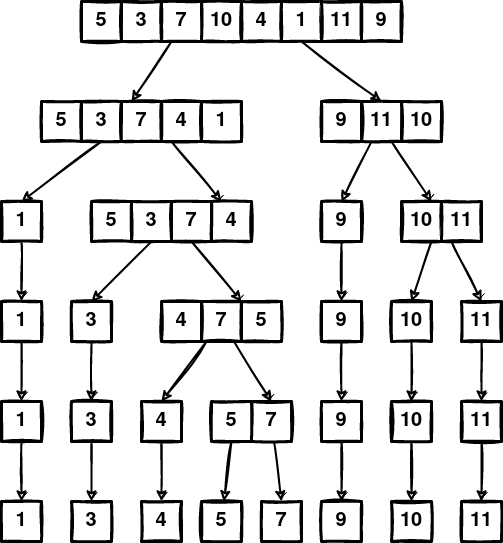
\includegraphics[width=0.6\linewidth]{images/quicksort/QuickSort}
\end{center}

{\small Nota: esto es sólo la idea general y no como exactamente funciona.}
\end{frame}

\section{QuickSort}
\begin{frame}[fragile]
 \frametitle{Esquemas de Partición}
\small QuickSort se basa en un esquema de particiones que puede ser implementado de variadas formas. Estos esquemas dependen de un valor pivote, que permite ordenar los sub-arreglos.\\
\bigskip
Generalmente, se comparan dos de las formas mas utilizadas:
\begin{itemize}
\item Forma Lomuto: Pivote al final. Facil implementación. Redundante.
\item Forma Hoare: Forma original. Pivote al inicio. Sofisticado. Muy eficiente.
\end{itemize}

En este curso veremos la forma original: El \textbf{Esquema de Hoare}.
\end{frame}

\begin{frame}[fragile]
 \frametitle{Partition: Hoare's Scheme}
\begin{center}
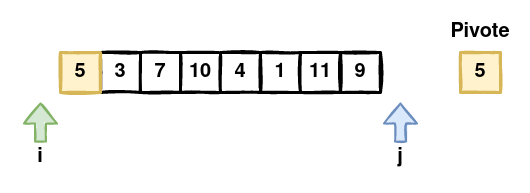
\includegraphics[width=0.8\linewidth]{images/quicksort/hoare1}
\end{center}
\end{frame}

\begin{frame}[fragile]
 \frametitle{Partition: Hoare's Scheme}
\begin{center}
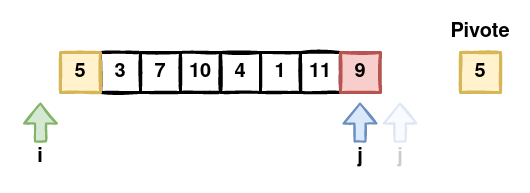
\includegraphics[width=0.8\linewidth]{images/quicksort/hoare2}
\end{center}
\end{frame}

\begin{frame}[fragile]
 \frametitle{Partition: Hoare's Scheme}
\begin{center}
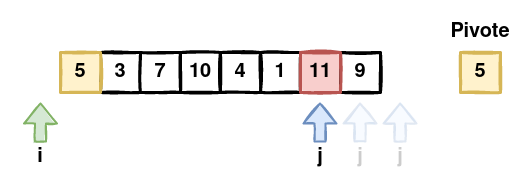
\includegraphics[width=0.8\linewidth]{images/quicksort/hoare3}
\end{center}
\end{frame}

\begin{frame}[fragile]
 \frametitle{Partition: Hoare's Scheme}
\begin{center}
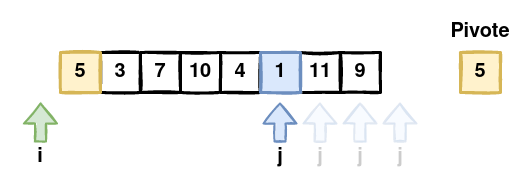
\includegraphics[width=0.8\linewidth]{images/quicksort/hoare4}
\end{center}
\end{frame}

\begin{frame}[fragile]
 \frametitle{Partition: Hoare's Scheme}
\begin{center}
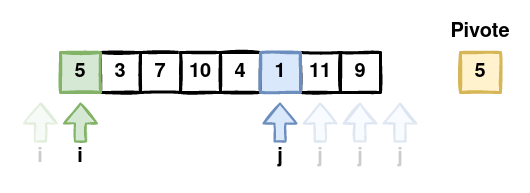
\includegraphics[width=0.8\linewidth]{images/quicksort/hoare5}
\end{center}
\end{frame}


\begin{frame}[fragile]
 \frametitle{Partition: Hoare's Scheme}
\begin{center}
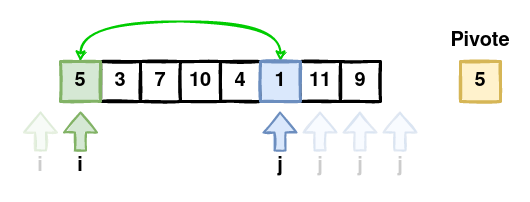
\includegraphics[width=0.8\linewidth]{images/quicksort/hoare6}
\end{center}
\end{frame}

\begin{frame}[fragile]
 \frametitle{Partition: Hoare's Scheme}
\begin{center}
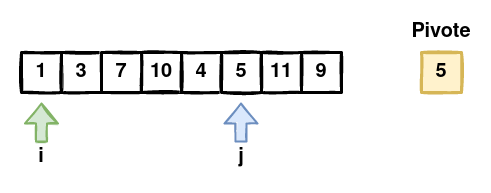
\includegraphics[width=0.8\linewidth]{images/quicksort/hoare7}
\end{center}
\end{frame}

\begin{frame}[fragile]
 \frametitle{Partition: Hoare's Scheme}
\begin{center}
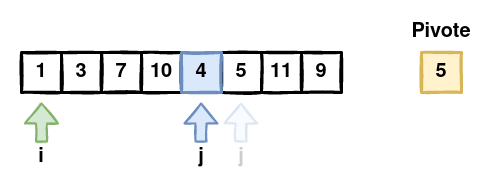
\includegraphics[width=0.8\linewidth]{images/quicksort/hoare8}
\end{center}
\end{frame}


\begin{frame}[fragile]
 \frametitle{Partition: Hoare's Scheme}
\begin{center}
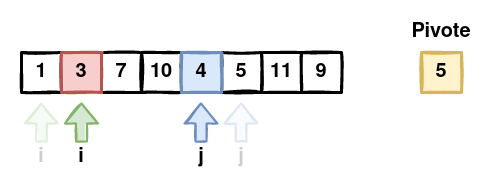
\includegraphics[width=0.8\linewidth]{images/quicksort/hoare9}
\end{center}
\end{frame}

\begin{frame}[fragile]
 \frametitle{Partition: Hoare's Scheme}
\begin{center}
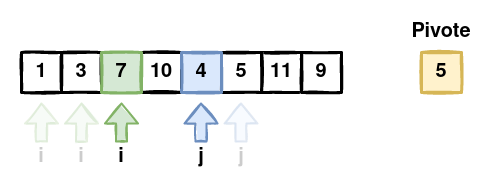
\includegraphics[width=0.8\linewidth]{images/quicksort/hoare10}
\end{center}
\end{frame}

\begin{frame}[fragile]
 \frametitle{Partition: Hoare's Scheme}
\begin{center}
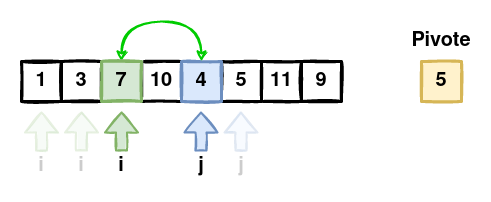
\includegraphics[width=0.8\linewidth]{images/quicksort/hoare11}
\end{center}
\end{frame}

\begin{frame}[fragile]
 \frametitle{Partition: Hoare's Scheme}
\begin{center}
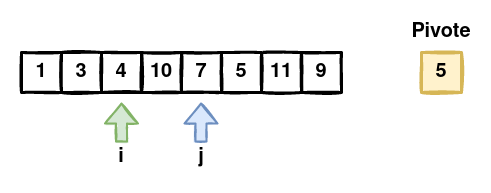
\includegraphics[width=0.8\linewidth]{images/quicksort/hoare12}
\end{center}
\end{frame}

\begin{frame}[fragile]
 \frametitle{Partition: Hoare's Scheme}
\begin{center}
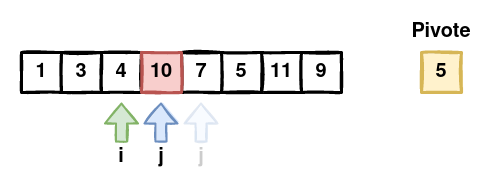
\includegraphics[width=0.8\linewidth]{images/quicksort/hoare13}
\end{center}
\end{frame}

\begin{frame}[fragile]
 \frametitle{Partition: Hoare's Scheme}
\begin{center}
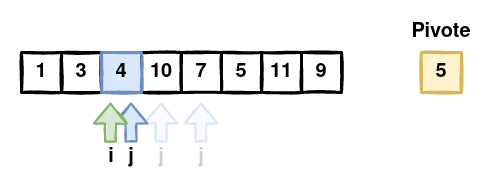
\includegraphics[width=0.8\linewidth]{images/quicksort/hoare14}
\end{center}
\end{frame}

\begin{frame}[fragile]
 \frametitle{Partition: Hoare's Scheme}
\begin{center}
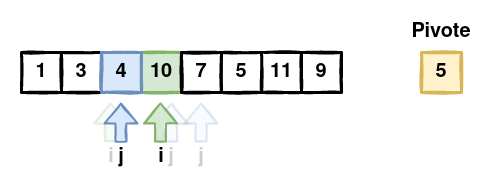
\includegraphics[width=0.8\linewidth]{images/quicksort/hoare15}
\end{center}
\end{frame}

\begin{frame}[fragile]
 \frametitle{Partition: Hoare's Scheme}
\begin{center}
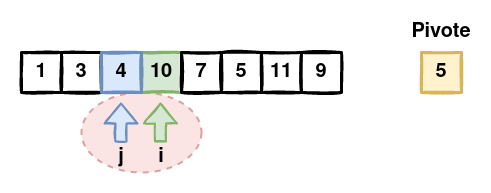
\includegraphics[width=0.8\linewidth]{images/quicksort/hoare16}
\end{center}
\end{frame}

\begin{frame}[fragile]
 \frametitle{Partition: Hoare's Scheme}
\begin{center}
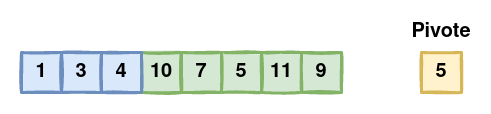
\includegraphics[width=0.8\linewidth]{images/quicksort/hoare17}
\end{center}
\end{frame}

\begin{frame}[fragile]
 \frametitle{Partition: Hoare's Scheme}
\begin{center}
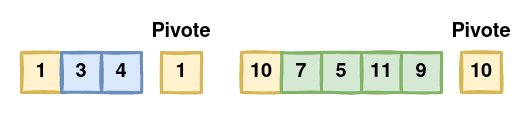
\includegraphics[width=0.8\linewidth]{images/quicksort/hoare18}
\end{center}
\end{frame}

\begin{frame}[fragile]
 \frametitle{Partition: Hoare's Scheme}

\begin{exampleblock}{Partition}
\begin{lstlisting}[language=C, basicstyle=\tiny, escapeinside={|}{|}]
int partition(int arr[], int inicio, int fin){
    int pivote = arr[inicio];
    int i = inicio - 1, j = fin + 1, temp;
 
    while (i<j){
        do{
            i++;
        }while (arr[i] < pivote);
 
        do{
            j--;
        }while (arr[j] > pivote);

	if(j<=i)
		break;
 
	temp = arr[i];
	arr[i] = arr[j];
	arr[j] = temp;
    }

    return j;
}
\end{lstlisting}
\end{exampleblock}
\end{frame}

\begin{frame}[fragile]
 \frametitle{QuickSort}
\small Quicksort en sí es un procedimiento sencillo.

\begin{exampleblock}{QuickSort}
\begin{lstlisting}[language=C, basicstyle=\tiny, escapeinside={|}{|}]
void quickSort(int arr[], int inicio, int fin){
    if (inicio < fin) {
        
	int corte = partition(arr, inicio, fin);
 
        quickSort(arr, inicio, corte);
        quickSort(arr, corte + 1, fin);
    }
}
\end{lstlisting}
\end{exampleblock}
\end{frame}

\begin{frame}[fragile]
 \frametitle{QuickSort}
\small Apliquemos QuickSort sobre el siguiente arreglo:
\begin{center}
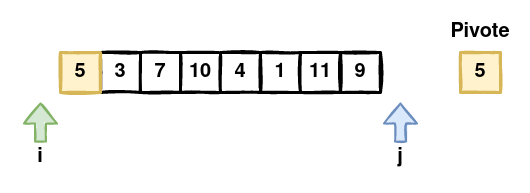
\includegraphics[width=0.8\linewidth]{images/quicksort/hoare1}
\end{center}
\end{frame}

\begin{frame}[fragile]
 \frametitle{QuickSort Aleatorizado}
\small ¿Cuál es el peor escenario de QuickSort?\\

Es cuando siempre nos queda una partición de 1 y otra de n-1. 
\begin{itemize}
\item Siempre tendremos que practicamente recorrer completamente el arreglo.
\item La recursión no será de largo $\log n$ sino $n$.
\item Por lo tanto la complejidad en el peor escenario es $\mathcal{O}(n^2)$.
\item El caso de la mala suerte (literal).
\end{itemize}

Para evitar eso, la elección del pivote se hace aleatoria, de esa forma el tiempo \textbf{esperado} (concepto estadístico) del peor escenario es $\mathcal{O}(n \log n)$. (Nota: el peor caso sigue siendo $\mathcal{O}(n^2)$).
\end{frame}


\begin{frame}[fragile]
 \frametitle{QuickSort Aleatorizado}
\begin{exampleblock}{QuickSort Aleatorizado}
\begin{lstlisting}[language=C, basicstyle=\tiny, escapeinside={|}{|}]
void quickSort(int arr[], int inicio, int fin){
    if (inicio < fin) {
        
	int corte = random_partition(arr, inicio, fin);
 
        quickSort(arr, inicio, corte);
        quickSort(arr, corte + 1, fin);
    }
}
\end{lstlisting}
\end{exampleblock}
\end{frame}

\begin{frame}[fragile]
 \frametitle{QuickSort Aleatorizado}
\begin{exampleblock}{Random Partition}
\begin{lstlisting}[language=C, basicstyle=\tiny, escapeinside={|}{|}]
int random_partition(int arr[], int inicio, int fin){
    int index = rand() % (fin + 1);
    int pivote = arr[index];
    int i = inicio - 1, j = fin + 1, temp;
 
    while (i<j){
        do{
            i++;
        }while (arr[i] < pivote);
 
        do{
            j--;
        }while (arr[j] > pivote);

	if(j<=i)
		break;
	 
	temp = arr[i];
	arr[i] = arr[j];
	arr[j] = temp;
    }

    return j;
}
\end{lstlisting}
\end{exampleblock}
\end{frame}

\begin{frame}[fragile]
 \frametitle{Ejercicios}
\begin{itemize}
\item Programa y dibuje la operación \texttt{partition} sobre el arreglo $A = \{13; 19; 9; 5; 12; 8; 7; 4; 21; 2; 6; 11\}$.
\item ¿Qué valor retorna \texttt{partition} cuando todos los elementos del arreglo son iguales?
\item ¿Cuál es el tiempo de ejecución de \texttt{QuickSort} cuando todos los elementos del arreglo son iguales?
\end{itemize}
\end{frame}

\end{document}
